\documentclass[10pt] {article}
\usepackage{fourier}
\author{Ankit Goyal \\ankit@cs.utexas.edu \\ CS380L}
\title{Lab 1: Scheduling}
\date{\today}	
\usepackage{full page}
\usepackage{minted} % to insert code
\usepackage{hyperref, url}
\usepackage{listings}
\usepackage{graphicx}
\usepackage{caption}
\usepackage{subcaption}
\usepackage{amsmath}
%\usepackage{amsmath, enumerate, url, ulem, algorithmic, polynom, subfig}

\begin{document}
\maketitle
%----------------------------------------------------------------------------------------
%  Specs
%----------------------------------------------------------------------------------------

\section{Setup}
\subsection{Hardware}
\textbf{Host Processor}: 64 bit 4 core Intel(R) Xeon(R) CPU E3-1270 V2 @ 3.50GHz\\
\textbf{Host Memory}: 16GB \\
\textbf{HyperThreading}: Yes \\
\textbf{Logical CPUs after Hyperthreading}: 8

\subsection{Software}
\textbf{Host Operating System}: Ubuntu with 3.13.0-34-generic 64 bit kernel.\\
\textbf{libcgroup.h} used for managing cgroups programatically.\\
\textbf{cityhash.h} c++ version from Google, used to calculate 128bit Hash values.

%----------------------------------------------------------------------------------------
%  Qemu Command Line
%----------------------------------------------------------------------------------------

\section{Single Process Hashing}

Single process computed about 722000 Hashes in 5 seconds.

%----------------------------------------------------------------------------------------
%  DMESG output
%----------------------------------------------------------------------------------------

\section{Multi Process Hashing}

\begin{table}
\centering
\begin{tabular}{ |c|c| } 
 \hline
\textbf{Number of Hashing Processes} & \textbf{Total Time} \\
\hline
4 & 5.515 \\ 
\hline
8 & 8.056\\
\hline
16 & 16.113\\
\hline
32 & 32.229\\
\hline
\end{tabular}
\caption{Showing increase in total time with number of hashing processes.}
 \label{table:hyperthrd}
\end{table}


\paragraph{Hyperthreading}
The processor has 4 physical cores and 8 logical cores (due to Hyperthreading). Table \ref{table:hyperthrd} shows that the rate of increase in total time is less when threads are increased from 4 to 8 than when increasing from 8 to 16. Hyperthreading is better than no Hyperthreading but not as better as extra physical cores. Note there are no background processes running.

%----------------------------------------------------------------------------------------
%  N vs N+1 Table
%----------------------------------------------------------------------------------------




\paragraph{N vs N+1 Processes}

Table \ref{table:nvsnplusone} shows the total time taken, throughput and fairness for (8 hashing, 8 background) and (8 hashing, 9 background) processes. Total time is the average value taken over 5 different runs. Throughput in (8 hashing, 8 background) is slightly higher than the throughput in (8 hashing, 9 background) since there are more number of processes to schedule.

\section{Throughput}

\subsection{\texttt{sched\_setaffinity} }

Using \texttt{sched\_setaffinity}, we attach each hashing process to a specific CPU. CPU Affinity improves cache performance since whenever a processor adds a line to its cache, all other processors needs to invalidate the data in their cache. In certain cases there could be huge improvements in performance due to affinity. The scheduler in 2.5 exhibit excellent natural affinity and prevents bouncing of a process from one CPU to another. CPU affinity could be very effective in case data is shared among different threads (in our case there's no sharing).\\

\noindent Figure \ref{fig:cpu_affinity} shows the effect of \texttt{sched\_setaffinity} in both (8 Hashing, 8 Background) and (8 Hashing, 9 Background processes). In both cases the throughput increased by 10.9\% and 9.5\% respectively.

\begin{table}
\centering
\begin{tabular}{ |c|c|c|c|c| } 
 \hline
\textbf{Hashing Processes \#} & \textbf{Background Processes \#} & \textbf{Total Time} & \textbf{Throughput} & \textbf{max deviation from mean (fairness)}\\
\hline
8 & 8 & 15.2418 & 0.5249 & 0.968625\\ 
\hline
8 & 9 & 15.5910 & 0.5131 & 0.70925\\
\hline
\end{tabular}
\caption{Throughput for different number of background and hashing processes.}
\label{table:nvsnplusone}
\end{table}


\begin{figure}[ht!]
\centering
\begin{subfigure}{.5\textwidth}
  \centering
  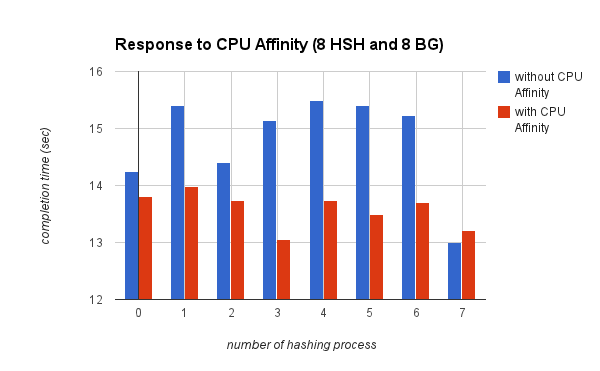
\includegraphics[width=\linewidth]{./cpu_agg_8_8.png}
  \caption{}
  \label{fig:sub1}
\end{subfigure}%
\begin{subfigure}{.5\textwidth}
  \centering
  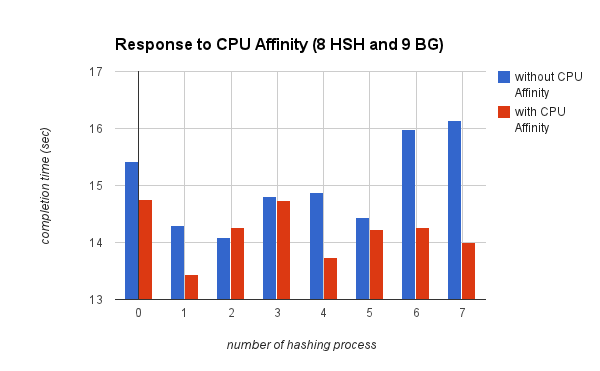
\includegraphics[width=\linewidth]{cpu_aff_8_9.png}
  \caption{}
  \label{fig:sub2}
\end{subfigure}
\caption{Response to CPU affinity: \textbf{\texttt{completion time}}  vs  \textbf{\texttt{hashing process number}}}
\label{fig:cpu_affinity}
\end{figure}

\subsection{\texttt{cgroups} }
Control Groups allow you to allocate resources - such as CPU time, system memory, network bandwidth - among user defined group of tasks (processes) running on the system. Using cgroups we can increase the amount of CPU available for hashing processes, which can significantly improve the throughput.

\noindent To increase \texttt{cpu.share} for hashing processes, a new cgroup for each process was created under the subsystem CPU. The \texttt{cpu.share} for all the tasks in these cgroups was increased to \texttt{2048} (default value is 1024). As a result all the hashing processes get twice the amount of cpu than other processes with default cgroups (background processes belong to default cgroups).

Figure \ref{fig:cgrp} shows relative time taken by each process with and without cgroups (and sched\_affinity). Throughput  was increased by 79.5\%, since the CPU was given twice to hashing processes than the background processes. It doesn't seem very useful to talk about fairness here, since we deliberately increased the CPU share and tied each hashing process to a different logical CPU.

\begin{figure}[ht!]
\centering
\begin{subfigure}{.5\textwidth}
  \centering
  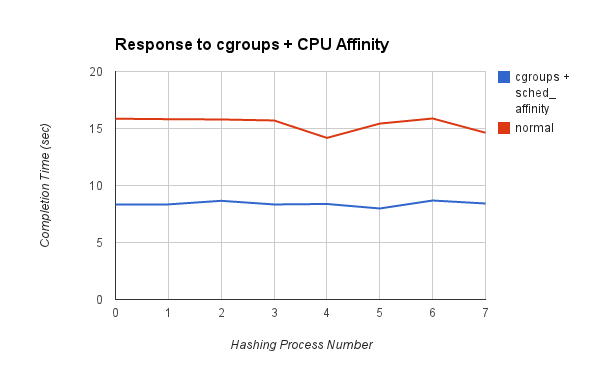
\includegraphics[width=\linewidth]{cgroup_affinity_8_9.png}
  \caption{}
  \label{fig:sub1}
\end{subfigure}%
\begin{subfigure}{.5\textwidth}
\centering

\begin{tabular}{ |c|c|c| } 
\hline
\textbf{Type} & \textbf{Total Time (sec)} & \textbf{Throughput} \\
\hline
normal & 15.5910 & 0.5131\\ 
\hline
cgroup+affinity &  8.684 & 0.9212 \\
\hline
\end{tabular}
\caption{}
\label{table:nvsnplusone}
  \label{fig:sub2}
\end{subfigure}
\caption{\textbf{Response to CPU affinity + cgroups}. (a) Relative time taken by each process with and without cgroup + affinity, (b) Throughput increase of 79.5\% for cgroup + affinity}
\label{fig:cgrp}
\end{figure}

\section{Fairness}


\noindent \textbf{Time Spent on the lab \ensuremath{\approx}14 hours} 

\section{References:}
1. \url{http://www.linuxjournal.com/article/6799}  \\
2. \url{http://www.makelinux.net/books/lkd2/ch10lev1sec5} \\
3. \url{http://linux.die.net/man/4/rtc} \\
4. \url{http://linux.die.net/man/4/urandom}

\end{document}